% AISIGH-SD 2026 (IEEE, CMT). IEEEtran conference, two-column. Overleaf: pdfLaTeX, no shell-escape.
% NOT anonymous. Hard limit 8 pages (6 standard; 7-8 paid over-length). PDF only, no supplementary file.
% Prose is written by the authors from paper/aisigh/briefs/. Every \placeholder{} must be gone before submission
% (python3 scripts/check_paper.py fails while any remains).
\documentclass[conference]{IEEEtran}
\IEEEoverridecommandlockouts
\usepackage{cite}
\usepackage{amsmath,amssymb}
\usepackage{graphicx}
\usepackage{booktabs}
\usepackage{url}
\usepackage{xcolor}
\newcommand{\placeholder}[1]{\textcolor{red}{\textbf{[#1]}}}

\begin{document}

\title{\placeholder{TITLE (authors)}}

\author{\IEEEauthorblockN{Karan Lokhande}
\IEEEauthorblockA{SVKM's NMIMS Mukesh Patel School of\\ Technology Management \& Engineering\\ Mumbai, India\\ \placeholder{email}}
\and
\IEEEauthorblockN{Akash Goyal}
\IEEEauthorblockA{SVKM's NMIMS Mukesh Patel School of\\ Technology Management \& Engineering\\ Mumbai, India\\ \placeholder{email}}
\and
\IEEEauthorblockN{Meer Magia}
\IEEEauthorblockA{SVKM's NMIMS Mukesh Patel School of\\ Technology Management \& Engineering\\ Mumbai, India\\ \placeholder{email}}
% Author order confirmed by the corresponding author (2 Oct 2026); fixed at submission (not anonymous).
}

\maketitle

\begin{abstract}
\placeholder{ABSTRACT: see briefs/00_abstract.md}
\end{abstract}

\begin{IEEEkeywords}
\placeholder{keywords}
\end{IEEEkeywords}

\section{Introduction}\label{sec:intro}
% CONTENT BRIEF: briefs/01_intro.md
\placeholder{SECTION TEXT (Introduction): authors write from briefs/01_intro.md}
\placeholder{required citations:}~\cite{gokhan2024regnlp,obliqamp,aueb2025rirag,indiafinbench,rbi}


\section{Related Work}\label{sec:related}
% CONTENT BRIEF: briefs/02_related.md
\placeholder{SECTION TEXT (Related Work): authors write from briefs/02_related.md}
\placeholder{required citations:}~\cite{gokhan2024regnlp,obliqamp,gokhan2025riragtask,repass,aueb2025rirag,indiafinbench,bm25s,bge,sbert,rrf}


\section{Corpus and Benchmark Construction}\label{sec:corpus}
% CONTENT BRIEF: briefs/03_corpus.md
\placeholder{SECTION TEXT (Corpus and Benchmark Construction): authors write from briefs/03_corpus.md}
\placeholder{required citations:}~\cite{rbi,bge}
% GENERATED by scripts/build_paper_tables_final.py from reports/results_v2.json. Do not edit numbers by hand.
\begin{table}[t]
\centering
\caption{RBI-ObliBench at a glance.}
\label{tab:benchmark}
\footnotesize
\setlength{\tabcolsep}{3pt}
\begin{adjustbox}{max width=\columnwidth}
\begin{tabular}{ll}
\toprule
Component & Size \\
\midrule
Corpus & 381 Directions; 76,188 paragraphs; 11 regulated classes \\
T1 (RQ1, RQ2) & 106 validated of 123 sampled; 412 class units \\
T2 (RQ1) & 291 / 53 / 25 queries (three relevance sets) \\
T3 & 52 items (of 60 built) \\
T4 (RQ3) & 30 questions $\times$ 4 answer types \\
\bottomrule
\end{tabular}
\end{adjustbox}
\end{table}

\begin{figure}[t]\centering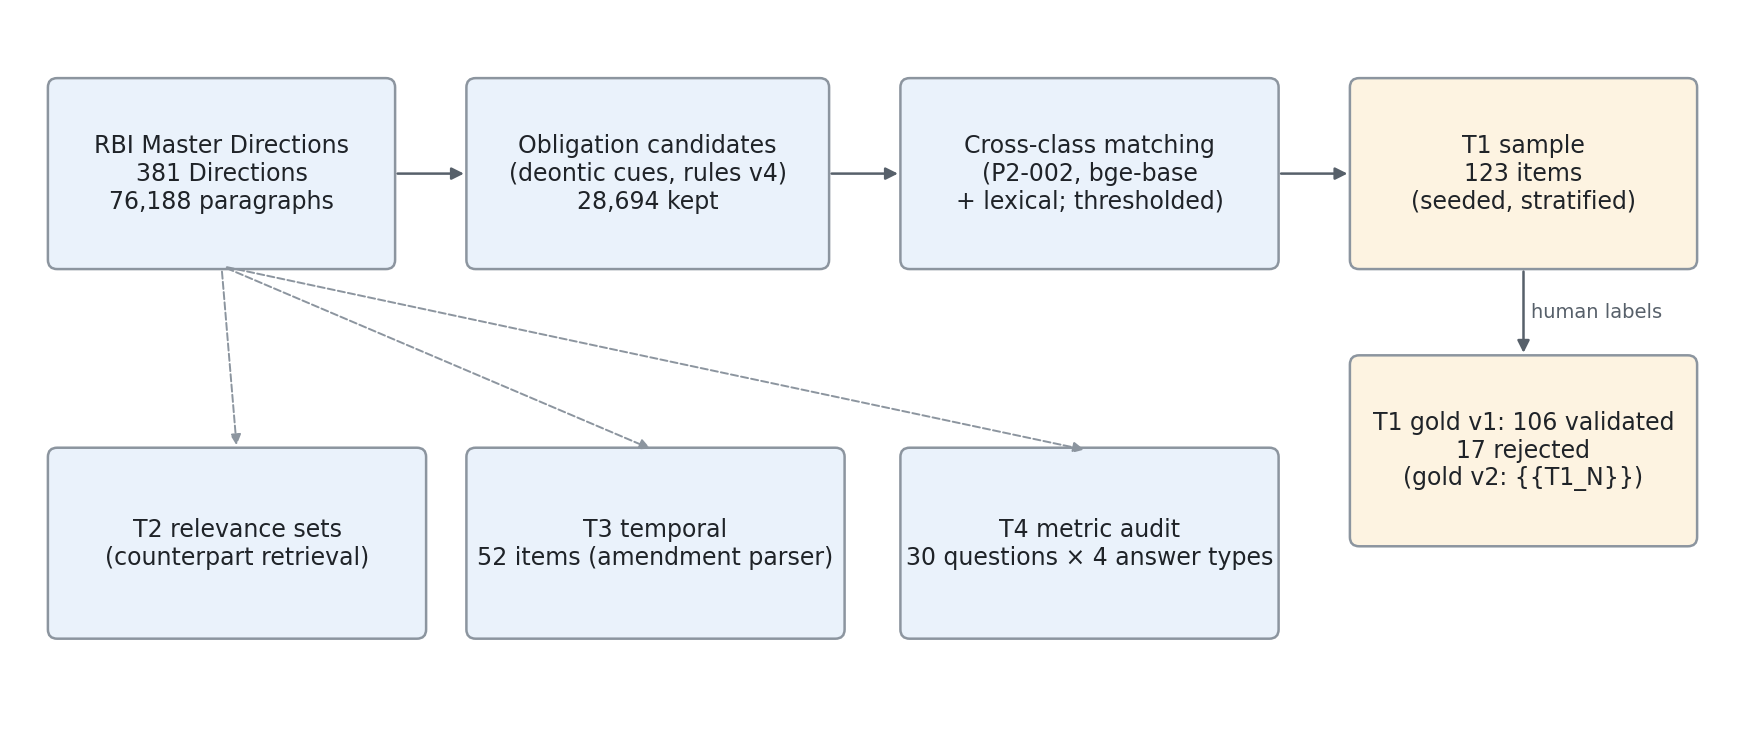
\includegraphics[width=\columnwidth]{figures/fig1_benchmark_construction.png}\caption{\placeholder{caption: benchmark construction}}\label{fig:construction}\end{figure}

\section{Annotation and Reliability}\label{sec:annotation}
% CONTENT BRIEF: briefs/04_annotation.md
\placeholder{SECTION TEXT (Annotation and Reliability): authors write from briefs/04_annotation.md}
\placeholder{required citations:}~\cite{fleiss1971,cohen1960,efron1979,wilson1927}
\begin{figure*}[t]\centering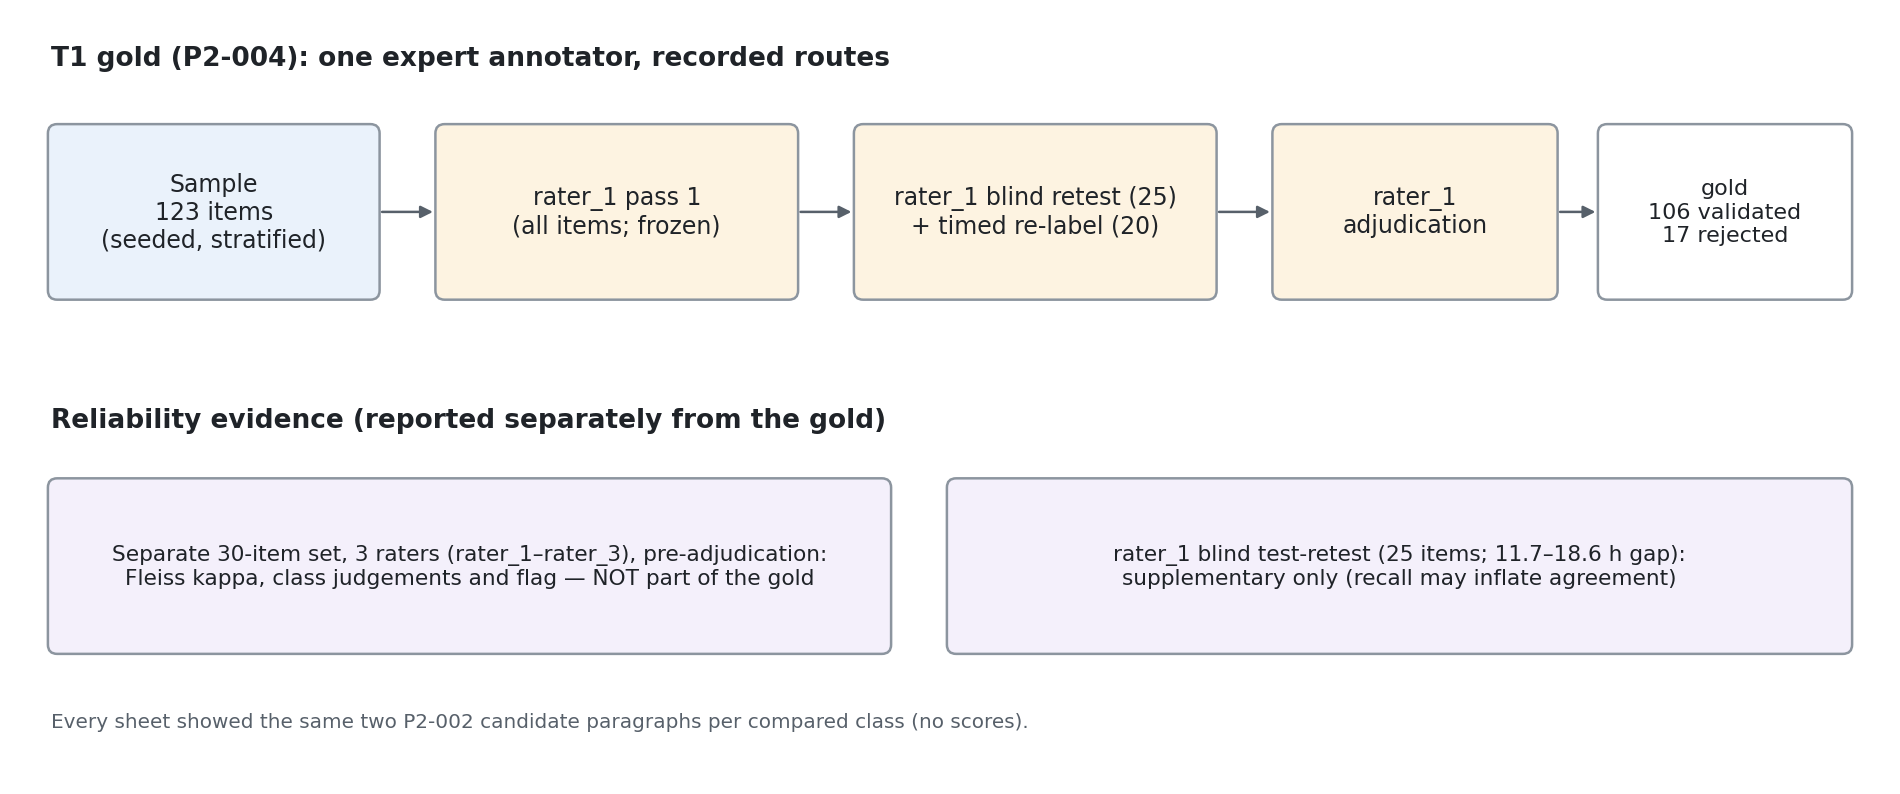
\includegraphics[width=0.9\textwidth]{figures/fig2_annotation_provenance.png}\caption{\placeholder{caption: annotation and provenance}}\label{fig:provenance}\end{figure*}
% GENERATED by scripts/build_paper_tables_final.py from reports/results_v2.json. Do not edit numbers by hand.
\begin{table*}[t]
\centering
\caption{Reliability evidence: $\kappa$ [95\% bootstrap CI] (items). Neither row is computed on the gold items.}
\label{tab:reliability}
\footnotesize
\setlength{\tabcolsep}{3pt}
\begin{adjustbox}{max width=\textwidth}
\begin{tabular}{lccc}
\toprule
Evidence & Class judgement & Flag & Not-obligation \\
\midrule
Separate 30-item set, 3 raters (Fleiss) & 0.774 [0.645, 0.886] (20) & 0.571 [0.289, 0.807] (20) & 0.392 [-0.015, 0.689] (30) \\
rater\_1 blind retest (11.7--18.6 h; Cohen) & 0.550 [0.333, 0.752] (20) & 0.426 [0.091, 0.730] (20) & 0.702 [0.000, 1.000] (25) \\
\bottomrule
\end{tabular}
\end{adjustbox}
\par\smallskip{\scriptsize The 30-item set was drawn outside the T1 sample; the gold is single-expert. The retest is supplementary: recall may inflate agreement.}
\end{table*}


\section{Tasks, Systems and Metrics}\label{sec:tasks}
% CONTENT BRIEF: briefs/05_tasks.md
\placeholder{SECTION TEXT (Tasks, Systems and Metrics): authors write from briefs/05_tasks.md}
\placeholder{required citations:}~\cite{gemini35fl,gptoss,bm25s,bge,rrf,nlideberta,debertav3,repass,gokhan2024regnlp,legalbert}


\section{Results}\label{sec:results}
% CONTENT BRIEF: briefs/06_results.md
\placeholder{SECTION TEXT (Results): authors write from briefs/06_results.md}
\placeholder{required citations:}~\cite{aueb2025rirag,repass}
% GENERATED by scripts/build_paper_tables_final.py from reports/results_v2.json. Do not edit numbers by hand.
\begin{table*}[t]
\centering
\caption{T2 counterpart retrieval, nDCG@10 [95\% CI].}
\label{tab:t2}
\footnotesize
\setlength{\tabcolsep}{3pt}
\begin{adjustbox}{max width=\textwidth}
\begin{tabular}{lccc}
\toprule
System & xclass\_t1 (291) & xclass\_p2002 (53) & supp\_p2003 (25) \\
\midrule
BM25 & 0.458 [0.424, 0.492] & 0.277 [0.194, 0.369] & 0.616 [0.462, 0.761] \\
Dense (bge) & 0.421 [0.385, 0.455] & 0.334 [0.252, 0.428] & 0.362 [0.212, 0.528] \\
Hybrid RRF & 0.443 [0.408, 0.478] & 0.319 [0.234, 0.414] & 0.504 [0.348, 0.673] \\
Hybrid $-$ source class & 0.464 [0.429, 0.497] & 0.337 [0.256, 0.429] & 0.504 [0.348, 0.673] \\
Class-aware hybrid & 0.894 [0.864, 0.922] & 0.741 [0.630, 0.844] & 0.675 [0.535, 0.811] \\
\bottomrule
\end{tabular}
\end{adjustbox}
\par\smallskip{\scriptsize The first two sets favour the dense retriever, the third BM25; the class-aware gain is partly by construction.}
\end{table*}

% GENERATED by scripts/build_paper_tables_final.py from reports/results_v2.json. Do not edit numbers by hand.
\begin{table*}[t]
\centering
\caption{T1 on the 106-item gold: 3-way flag Macro-F1, collapsed (absent vs present) Macro-F1, judgement Macro-F1, \textit{different} F1 (point estimate) and coverage.}
\label{tab:t1}
\footnotesize
\setlength{\tabcolsep}{3pt}
\begin{adjustbox}{max width=\textwidth}
\begin{tabular}{lcccccc}
\toprule
System & $n$ & 3-way F1 & Collapsed F1 & Judgement F1 & \textit{diff.} F1 & Coverage \\
\midrule
Majority (in-sample) & 106 & 0.219 [0.186, 0.246] & 0.465 [0.445, 0.483] & 0.227 [0.202, 0.248] & 0.000 & 1.000 [1.000, 1.000] \\
P2-002 candidates & 106 & 0.459 [0.381, 0.520] & 0.784 [0.671, 0.877] & 0.550 [0.512, 0.583] & 0.000 & 1.000 [1.000, 1.000] \\
Class-blind LLM & 106 & 0.602 [0.497, 0.700] & 0.766 [0.647, 0.873] & 0.664 [0.597, 0.726] & 0.321 & 1.000 [1.000, 1.000] \\
Class-aware LLM & 106 & 0.551 [0.445, 0.639] & 0.808 [0.685, 0.908] & 0.609 [0.553, 0.667] & 0.154 & 0.991 [0.972, 1.000] \\
Final agentic & 106 & 0.483 [0.385, 0.568] & 0.710 [0.590, 0.815] & 0.521 [0.470, 0.570] & 0.047 & 0.774 [0.689, 0.849] \\
Class-blind + verifier & 106 & 0.532 [0.431, 0.625] & 0.695 [0.572, 0.802] & 0.578 [0.520, 0.639] & 0.176 & 0.792 [0.708, 0.868] \\
Long-context (100K) & 102 & 0.509 [0.408, 0.600] & 0.819 [0.691, 0.917] & 0.551 [0.496, 0.604] & 0.074 & 1.000 [1.000, 1.000] \\
Structured comparator & 106 & 0.616 [0.512, 0.702]$^*$ & 0.838 [0.720, 0.926]$^*$ & 0.680 [0.622, 0.732] & 0.409 & 1.000 [1.000, 1.000] \\
\bottomrule
\end{tabular}
\end{adjustbox}
\par\smallskip{\scriptsize 2,000 item resamples. Collapsed F1 is the fair comparison with P2-002, which cannot express shared vs class-specific. $^*$Comparator flag derived from its judgements (v3.6 rule); its judgement metrics are the pre-registered ones. CIs not computed for the \textit{diff.} F1 column. Majority (in-sample) uses the gold distribution: a reference, not a deployable system. Abstentions are scored as errors, so the verifier's loss in F1 reflects both wrong answers and declined correct ones (coverage $-$0.217). Long-context items that exceeded the input cap are excluded rather than penalised, and every comparison with long-context is made on the same 102 items.}
\end{table*}

% GENERATED by scripts/build_paper_tables_final.py from reports/results_v2.json. Do not edit numbers by hand.
\begin{table}[t]
\centering
\caption{T3, T4 and ablations A--C (ON $-$ OFF), 95\% CI.}
\label{tab:t3t4}
\footnotesize
\setlength{\tabcolsep}{3pt}
\begin{adjustbox}{max width=\columnwidth}
\begin{tabular}{llc}
\toprule
 & Measure & Value \\
\midrule
T3 & status exact match, filter on (circular) & 1.000 [1.000, 1.000] \\
T3 & status exact match, filter off & 0.538 [0.404, 0.673] \\
T4 & concatenated $-$ genuine (RePASs) & +0.375 [+0.325, +0.427] \\
T4 & negated $-$ genuine & -0.322 [-0.390, -0.243] \\
T4 & off-topic $-$ genuine & -0.141 [-0.206, -0.080] \\
T4 & $\rho$(RePASs, human faithful) & 0.731 [0.535, 0.845] \\
T4 & $\rho$(RePASs, answers question) & 0.008 [-0.323, 0.339] \\
A & class filter: T2 nDCG@10 (xclass\_t1) & +0.451 [+0.421, +0.481] \\
A & class filter (with verifier): T1 3-way F1 & -0.049 [-0.133, +0.036] \\
B & temporal filter: T3 exact match & +0.462 [+0.327, +0.596] \\
C & verifier: T1 3-way F1 & -0.068 [-0.132, -0.012] \\
C & verifier: T4 abstention & +0.393 [+0.214, +0.571] \\
\bottomrule
\end{tabular}
\end{adjustbox}
\par\smallskip{\scriptsize T3 gold and filter share one parser. T4 verdicts are pre-registered; unchanged without the 2 bad questions.}
\end{table}


\section{Targeted Experiment: Structured Comparison}\label{sec:comparator}
% CONTENT BRIEF: briefs/07_comparator.md
\placeholder{SECTION TEXT (Targeted Experiment: Structured Comparison): authors write from briefs/07_comparator.md}
\placeholder{required citations:}~\cite{gemini35fl}


\section{Discussion}\label{sec:discussion}
% CONTENT BRIEF: briefs/08_discussion.md
\placeholder{SECTION TEXT (Discussion): authors write from briefs/08_discussion.md}


\section{Limitations}\label{sec:limitations}
% CONTENT BRIEF: briefs/09_limitations.md
\placeholder{SECTION TEXT (Limitations): authors write from briefs/09_limitations.md}


\section{Ethics, Licensing and AI Use}\label{sec:ethics}
% CONTENT BRIEF: briefs/10_ethics.md
\placeholder{SECTION TEXT (Ethics, Licensing and AI Use): authors write from briefs/10_ethics.md}
\placeholder{Data and code availability: Zenodo DOI}



\section*{Acknowledgment}
\placeholder{ACKNOWLEDGMENT + AI-use statement: see briefs/11_ai_use_ack.md}

\bibliographystyle{IEEEtran}
\bibliography{refs_verified}

\end{document}
